\documentclass{article} % Use an appropriate document class for your main document
\usepackage{tikz}
\usetikzlibrary{positioning, shapes.geometric}

\begin{document}

\begin{figure*}[t]
    \centering
    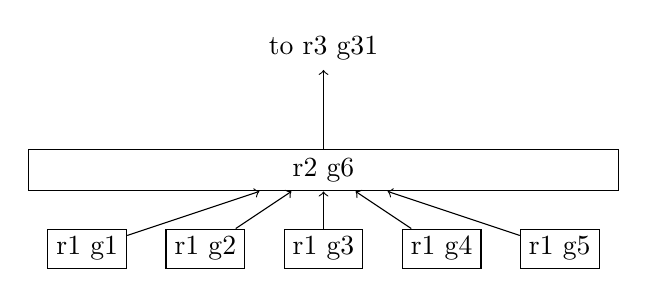
\begin{tikzpicture}[node distance=1cm and 1cm]
        % Bottom level blocks (5 participants)
        \foreach \x in {1,...,5} {
            \node[draw, rectangle, minimum width=1cm, minimum height=0.5cm] (P-\x) at (\x*1.5, 0) {};
            % Add "Rank X" text inside each block
            \node at (\x*1.5, 0) {r1 g\x};
        }

        % Single block for the game
        \node[draw, rectangle, minimum width=7.5cm, minimum height=0.5cm] (Game) at (4.5, 1) {r2 g6};

        % Connect participants to the game
        \foreach \x in {1,...,5}
            \draw[->] (P-\x) -- (Game);

        % Arrow pointing upwards from the top block with text "to r3"
        \draw[->] (Game.north) -- ++(0,1) node[above] {to r3 g31};
    \end{tikzpicture}
    \caption{Diagram illustrating the rank ladder. With minimum participant requirements of 5, 30 games are required to create a rank 3 game. Strong candidate would need only 2 wins to reach it.}
    \label{fig:game-connection}
\end{figure*}


\end{document}